% \iffalse meta-comment
% rubikrotation.dtx
%
% version 4.0
%
% Authors:   RWD Nickalls (dick@nickalls.org) 
%        and Apostolos Syropoulos (asyropoulos@yahoo.com)

% Copyright   03 March 2017  RWD Nickalls + A Syropoulos
%
% This work may be distributed and/or modified under the
% conditions of the LaTeX Project Public License, either
% version 1.3c of this license or (at your option) any
% later version. The latest version of this licence is in 
%
%       http://www.latex-project.org/lppl.txt
%
%<*readme>
%
% The rubikrotation package provides a collection of LaTeX commands and macros 
% for the typesetting of Rubik cube configurations and rotation 
% sequences using the TikZ graphic language.
%
% Please report errors or suggestions for improvement to
%
%         Dick Nickalls or Apostolos Syropoulos
%
% This package requires the basic TikZ package to be loaded already
%</readme>
%
%<*driver>
\listfiles
\documentclass{ltxdoc}
\IfFileExists{rubikrotation.sty}{\usepackage{rubikrotation}}{%
    \GenericWarning{rubikrotation.dtx}{Package file rubikrotation.sty not found.
    Documentation will be messed up!^^J
    (Generate rubikrotation.sty by (La)TeXing rubikrotation.ins, and then^^J
    process rubikrotation.dtx again)^^J}\stop
}%
\usepackage{ifpdf}
\usepackage{url,path}  %% for references and paths
\usepackage{graphicx}  %% for the two pdf figs
\usepackage{hypdoc}    %% for pdf bookmarks + hyperref documenting of packages
%%\OnlyDescription
\EnableCrossrefs
\PageIndex
\CodelineIndex
\CodelineNumbered
\RecordChanges
\setcounter{StandardModuleDepth}{1}
\begin{document}
  \DocInput{rubikrotation.dtx}
  \PrintChanges
  \PrintIndex
\end{document}
%</driver>
% \fi
%
%
% 
%%% \CheckSum{322}
%
%%% \CharacterTable
%%  {Upper-case    \A\B\C\D\E\F\G\H\I\J\K\L\M\N\O\P\Q\R\S\T\U\V\W\X\Y\Z
%%   Lower-case    \a\b\c\d\e\f\g\h\i\j\k\l\m\n\o\p\q\r\s\t\u\v\w\x\y\z
%%   Digits        \0\1\2\3\4\5\6\7\8\9
%%   Exclamation   \!     Double quote  \"     Hash (number) \#
%%   Dollar        \$     Percent       \%     Ampersand     \&
%%   Acute accent  \'     Left paren    \(     Right paren   \)
%%   Asterisk      \*     Plus          \+     Comma         \,
%%   Minus         \-     Point         \.     Solidus       \/
%%   Colon         \:     Semicolon     \;     Less than     \<
%%   Equals        \=     Greater than  \>     Question mark \?
%%   Commercial at \@     Left bracket  \[     Backslash     \\
%%   Right bracket \]     Circumflex    \^     Underscore    \_
%%   Grave accent  \`     Left brace    \{     Vertical bar  \|
%%   Right brace   \}     Tilde         \~}
%
%
%
% \title{%
%       \ifpdf\pdfbookmark[1]{Title}{Title}\else\fi%
%       The \rubikrotation\ package}
%
% \author{
%      RWD Nickalls (dick@nickalls.org) \\
%     A Syropoulos (asyropoulos@yahoo.com)
%       }
%  \date{This file describes version \RRfileversion\ (\RRfiledate)\\
%  \texttt{www.ctan.org/pkg/rubik}}
%  \maketitle
%
%  \begin{abstract}
%  The \rubikrotation\ package is a dynamic extension for  the 
%  \textsc{rubikcube} package (both are part of the Rubik `bundle'). 
%  This package provides  the \cmd{\RubikRotation} command which 
%  processes a sequence of Rubik rotation moves on-the-fly (using the Perl script
%  \texttt{rubikrotation.pl}), and returns the new Rubik cube  state (configuration).  
%  The \rubikrotation\ package  also provides  commands for saving the cube state 
%  to a file (\cmd{\SaveRubikState}), and for displaying any 
%  errors (\cmd{\ShowRubikErrors}).
%  \end{abstract}
% 
% 
% \begin{minipage}{11cm}
% \centering
% \ifpdf
%  \strut\hspace{6mm}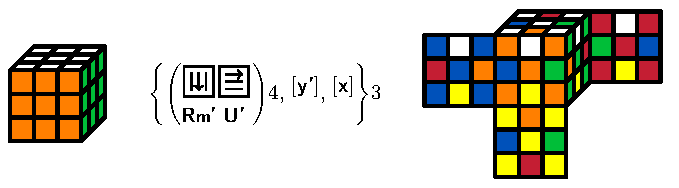
\includegraphics[width=10cm]{rubikrot-doc-figD.pdf}
% \else
% \fi
% \end{minipage}
% 
%
% \vspace{-1\baselineskip}
%
%  \tableofcontents
%
% \pagebreak
%
% \section{Introduction}
%
% The \rubikrotation\ package is a dynamic extension to the \textsc{rubikcube} package.
% It consists of a style option (\texttt{rubikrotation.sty}), a 
%  Perl script  (\texttt{rubikrotation.pl}).
% 
% The primary role of the \rubikrotation\ package is to  implement  a sequence of 
%  Rubik rotation moves on-the-fly using the \cmd{\RubikRotation} command.  
%  Consequently the \rubikrotation\  package requires access to the \TeX\ \texttt{write18} 
%  facility, which is enabled by using the \texttt{--shell-escape} command-line switch.
%  This allows command-line control of  the  Perl script, which is really the `engine' of 
%  this package.
%
%  The \rubikrotation\ package has been road-tested  on a Microsoft 
%  platform (MiKTeX and Strawberry Perl\,\footnote{`Strawberry Perl' 
%  (\texttt{http://strawberryperl.com}) is a free Perl 
%  environment for MS Windows, designed to be as close as possible to the Perl 
%  environment of Unix/Linux systems.}), on a Linux platform (Debian v8.2.0,  
%  {\TeX}Live 2016, and Perl v5.20.2), and on  a Solaris platform (OpenIndiana).
%
% The following  commands are made available  by  \texttt{rubikrotation.sty}:
% \begin{quote}
% \begin{verbatim}
%    \RubikRotation[]{}
%    \SaveRubikState
%    \CheckRubikState
%    \ShowRubikErrors
%    \SequenceName
%    \SequenceInfo
%    \SequenceShort
%    \SequenceLong
%\end{verbatim}
% \end{quote}
%
%
%  \section{Requirements}
% 
% The \rubikrotation\ package  requires the TikZ and the \textsc{rubikcube} packages.
% 
%
%   \section{Installation}
%
%  \subsection{Generating the files}
%
%  Place the file \texttt{rubikrotation.zip} into a temporary directory, and unzip it. 
% This will generate the following files:
%\begin{quote}
% \begin{verbatim}
% rubikrotation.ins
% rubikrotation.dtx
% rubikrotation.pdf     --this document
% rubikrotation.pl      --Perl script
% rubikrotationPL.pdf   --documentation of rubikrotation.pl
% rubikrotation.1       --manual file for rubikrotation.pl (`man' file)
% rubikrot-doc-figA.pdf
% rubikrot-doc-figB.pdf
% rubikrot-doc-figC.pdf
% rubikrot-doc-figD.pdf
%\end{verbatim}
%\end{quote}
% The main package documentation is the file \texttt{rubikrotation.pdf}.
% The documentation of the Perl program \texttt{rubikrotation.pl} is the file \texttt{rubikrotationPL.pdf} 
%
%  The  style option \texttt{rubikrotation.sty} is generated  by  running (pdf)\LaTeX\ on  
% the file \texttt{rubikrotation.ins}  as follows:
%\begin{quote}
%\begin{verbatim}
%   pdflatex  rubikrotation.ins 
%\end{verbatim}
%\end{quote}
% The documentation file (\texttt{rubikrotation.pdf}) is then generated using the following 
% sequence of steps\,\footnote{Since the documentation includes a complicated indexing 
% system as well as an index and hyperef links (the package \texttt{hypdoc}
%  is used), then a lot of pdflatex runs are required. Prior to the first run it is
% a good idea to delete any relevant \texttt{.toc}, \texttt{.aux}, \texttt{.out} files.}:
%\begin{quote}
% \begin{verbatim}
%  pdflatex    rubikrotation.dtx
%  pdflatex    rubikrotation.dtx
%  makeindex -s gind.ist  rubikrotation
%  makeindex -s gglo.ist -o rubikrotation.gls  rubikrotation.glo
%  pdflatex    rubikrotation.dtx
%  pdflatex    rubikrotation.dtx
%\end{verbatim}
%\end{quote}
%
%
% 
%  \subsection{Placing the files}
% \label{sec:placingfiles}
%
% Place the files either in a working directory, or where your system 
% will find them, e.g.,~in your \texttt{/texmf-local/} directory tree. 
% For example, on a Linux platform with a standard \TeX\ Directory Structure (TDS), then:
%
%\medskip
%{\noindent}*.sty  $\rightarrow$  \texttt{/usr/local/texlive/texmf-local/tex/latex/rubik/}
%{\newline}*.cfg  $\rightarrow$  \texttt{/usr/local/texlive/texmf-local/tex/latex/rubik/}
%{\newline}*.pdf  $\rightarrow$  \texttt{/usr/local/texlive/texmf-local/doc/rubik/}
%{\newline}*.pl  $\rightarrow$  \texttt{/usr/local/texlive/texmf-local/scripts/rubik/}
%
%\medskip
%{\noindent}\textsc{perl script}:\ \ Make the perl script  executable 
% (\texttt{chmod +x rubikrotation.pl}), and then
% rename the file as `rubikrotation' (i.e.,~with no file extension), and then place 
% the executable script into your current TeXLive binary directory, 
% e.g.,~\path!/user/local/texlive/YYYY/bin/i386-linux!.
%
% Sometimes the setting up of a simple one or two-line plain-text 
% configuration-file may be  useful or even necessary, depending on your system
% (see Section~\ref{sec:configfile} below). Such a file (if one exists) will 
% automatically be read by \texttt{rubikrotation.sty} providing the 
% file is named \texttt{rubikrotation.cfg}.
%
%\medskip
%{\noindent}\textsc{the `man' file}:\ \ On a Linux platform this manual file 
% (\texttt{rubikrotation.1}) would be  typically  located in the 
% directory \verb!/usr/share/man/man1!.
%
%\medskip
%{\noindent}\textsc{file database}:\ \ Finally, (depending on your system) update the 
% \TeX\ file database. 
% For example, on a Linux platform  this is achieved using the \texttt{texhash} command.
%
%\medskip
%{\noindent}\textsc{quick test}:\ \ To test that your system can now run the perl 
% script, just type at the command-line
%\begin{quote}
% \begin{verbatim}
%  rubikrotation  -h
%\end{verbatim}
%\end{quote}
% which should generate something like the following:
% \begin{verbatim}
% This is rubikrotation version 4.0
%       Usage: rubikrotation [-h] -i <input file> [-o <out file>]
%       where,
%       [-h]    gives this help listing
%       [-i]    creates specified input file
%       [-o]    creates specified output file
%       For documentation see: rubikrotation.pdf,
%       rubikrotationPL.pdf and  rubikcube.pdf
%\end{verbatim}
%
%
%       \section{Usage}
% \label{sec:usage}
% Load the  packages \texttt{rubikcube.sty}, 
%  \texttt{rubikrotation.sty} and \texttt{rubikpatterns.sty} in the \TeX\ file 
%  preamble  \textit{after} loading the TikZ package (all the  Rubik packages 
%  require the TikZ package); for example, as follows: 
%\begin{quote}
% \begin{verbatim}
% \usepackage{tikz}
% \usepackage{rubikcube,rubikrotation,rubikpatterns}
%\end{verbatim}
%\end{quote}
% and run (pdf)\LaTeX\ using the \texttt{--shell-escape} command-line option 
% (see the following section).
%
%
%
%   \subsection{Enabling the \TeX\ `shell' facility}
%   \label{sec:shellescape}
%
%  In order to access the  \TeX\  \cmd{\write18} syntax (so we can access system commands, 
%  and hence run the Perl script), 
% it is necessary to invoke  the \LaTeX\ engine (e.g.,~(pdf)\LaTeX\  or Lua\LaTeX) 
% using the \texttt{--shell-escape} command-line option; for example: 
%\begin{quote}
% \begin{verbatim}
% pdflatex  --shell-escape  filename.tex
%\end{verbatim}
%\end{quote}
% In practice, it is probably most convenient to  run this command via a 
% bash/batch file. For example, on a Linux platform  the following bash file 
% will run the file, show any errors, and  open the \textsc{pdf} using AcrobatReader.
%\begin{quote}
% \begin{verbatim}
% pdflatex  --shell-escape   filename.tex
% echo "...checking error file" 
% grep ERROR  ./rubikstateERRORS.dat
% acroread filename.pdf &
%\end{verbatim}
%\end{quote}
%  If the \LaTeX\ engine is  Lua\LaTeX, e.g.,
%\begin{quote}
% \begin{verbatim}
% lualatex  --shell-escape  filename.tex
%\end{verbatim}
%\end{quote}
%then  \texttt{rubikrotation.sty} will automatically load 
%  the recently developed  \textsf{shellesc} package in order to facilitate system access to  Perl 
%  (see Section~\ref{sec:CodePackageHeading}). See \textit{\LaTeX\ News}, issue~24, 
%  Feb~2016 for further details of the \textsf{shellesc} package.
%  Consequently, if you intend to use Lua\LaTeX\ then you will need to ensure your system
%  has access to the \textsf{shellesc} package (it can always be downloaded from CTAN directly).
%
%
%   \subsection{Configuration-file}
%   \label{sec:configfile}
%
%  A plain-text configuration-file with the name \texttt{rubikrotation.cfg} 
%  (if one exists) will automatically be  read  by \texttt{rubikrotation.sty}. 
%  The \rubikrotation\ package's facility to use a  configuration-file allows the 
%  user to  change not only (a)~the filename of the Perl script (\texttt{rubikrotation.pl}),
%  but also (b)~the command-line code used by \texttt{rubikrotation.sty} for calling the 
%  Perl script.  This~sort of fine-tuning can be very useful, and sometimes may 
%  even be necessary (depending on your system) for running the Perl script.
%
%  For example, on some systems it maybe preferable  to use a different \textsc{path}, 
%  file-name and/or  a different  command-line code to  call the script. 
%  Such~a configuration-file can also facilitate testing a new Perl script  having 
%  a different name and location.
%
%
%  \DescribeMacro{\rubikperlname}
%  \DescribeMacro{\rubikperlcmd}
% The configuration-file is essentially a convenient software vehicle for feeding  
% additional  \LaTeX\ code  to the  style option \texttt{rubikrotation.sty}, and hence 
% allows the contents of some commands to be easily adjusted and/or fine-tuned.
% For~the \rubikrotation\ package there are two particular macros we may wish to adjust.
% The~first is that  holding the filename of the Perl script, namely  
% \cmd{\rubikperlname}. The second is that holding the command-line call, 
% namely  \cmd{\rubikperlcmd}.
% The~default definitions in \texttt{rubikrotation.sty}  (which assume the Perl 
% script is executable), are as follows:  (they are detailed in 
% Section~\ref{sec:usefulcommands})
%\begin{quote}
%\begin{verbatim}
% \newcommand{\rubikperlname}{rubikrotation}
% \newcommand{\rubikperlcmd}{\rubikperlname\space%
%                     -i rubikstate.dat -o rubikstateNEW.dat}
%\end{verbatim}
%\end{quote}
% Note the need here (in the second macro) to use  \cmd{\space} on the end of 
%   (\cmd{\rubikperlname}) in  order to force a following 
% space---i.e.,~before the  first command-line argument. The following examples 
% illustrate how the configuration-file may be used.
%
% \medskip
% {\noindent}\textsc{example~1}:\ \ Suppose we wish to test out 
% a slightly modified  Perl script  
% with the  working (executable) name \texttt{rubikrotationR77}. In this case we 
% simply  create, in the local working  directory, a plain-text configuration-file 
% (it \textit{must} be named exactly \texttt{rubikrotation.cfg})  and contains just 
% the following line:
%\begin{quote}
%\begin{verbatim}
%\renewcommand{\rubikperlname}{rubikrotationR77}
%\end{verbatim}
%\end{quote}
%
% \medskip
% {\noindent}\textsc{example~2}:\ \ Alternatively, suppose we wish to test out 
% a new Perl script with the (non-executable) name \texttt{rubikrotationR55.pl}.
% Now, in this particular case  we  will need to run the script using a 
% slightly different  command, namely,
% {\linebreak}\texttt{perl  rubikrotationR55.pl ...}, and consequently we 
% need to  implement \textit{both} these  changes (of name and  command) in 
% the configuration-file,  as follows:
%\begin{quote}
%\begin{verbatim}
%\renewcommand{\rubikperlname}{rubikrotationR55.pl}
%\renewcommand{\rubikperlcmd}{perl  \rubikperlname\space\%
%                     -i rubikstate.dat   -o rubikstateNEW.dat}
%\end{verbatim}
%\end{quote}
%{\noindent}Remember to make sure the PATH associated with the command is also correct.
%
%
%{\noindent\textsc{placing the configuration-file}:\ \ The simplest arrangement is
% just to include the \texttt{.cfg} file in the working  directory.
% Alternatively, the \texttt{.cfg} file could be placed in the \texttt{/texmf-local/}
% directory tree (say, in \path!/usr/local/texlive/texmf-local/tex/latex/rubik/!), 
% but in this case one would then have to be careful to specify the 
% correct PATH for everything in order to enable your system to find all the 
% various components etc.
%
% Note that you can, of course,  have several \texttt{.cfg} files, since the system will 
% read only  one such file (the first one it finds starting with the current working 
% directory). Consequently, it may be useful to have  one \texttt{.cfg} file in 
% your \texttt{/texmf-local/} dir (for running the standard  Rubik package), 
% and another (different) \texttt{.cfg} file in your `test' directory.
%
% 
%   \section{Commands}
%
%  The \textit{only} `Rubik bundle'  commands which \textit{must} be used inside a TikZ picture 
%  environment are the \cmd{\Draw...} commands (these are all provided by 
%  the \textsc{rubikcube} package), although most  commands  can be placed
%  inside a TikZ environment if you wish. 
%
%  However, using commands which influence the Rubik colour state 
% (e.g.,~the \cmd{\RubikRotation} command) outside the  \texttt{tikzpicture}, 
% \texttt{minipage} or \texttt{figure} environments
%  generally  offers maximum  flexibility, since the effects of such commands when 
% used inside these environments remain `local' to  the  environment, and are not 
%  therefore accessible  outside that \textit{particular} environment 
% (see also Section~4.1 in the \textsc{rubikcube} documentation).
%
%  Conversely, the only \rubikrotation\  command which should \textit{not}
%  be used inside a TikZ environment is the \cmd{\ShowRubikErrors} command 
%  (see the notes on this command below). 
% 
%
%
%
%   \subsection[RubikRotation]{\cmd{\RubikRotation} command}
%       \label{sec:rubikrotationcmd}
%
%  \DescribeMacro{\RubikRotation}
% The  \cmd{\RubikRotation}\oarg{integer}\marg{comma-separated sequence}  
% command processes  a sequence of rotation codes, and returns 
% the final state. The inverse sequence can also be 
% implemented (see  \textbf{Inverse} below).
%
%
% The first (optional) argument \oarg{integer}  of the \cmd{\RubikRotation} command  is the number
% of times the whole command itself should be repeated; for example
% as follows: \verb!\RubikRotation[2]{...}!.
%
% The second (mandatory) argument consists of a comma-separated sequence
% of  rotation codes, e.g.,~\texttt{U, D2}, which may be encoded as a macro. In addition, there 
% may be additional comma-separated macros and optional \verb![name]!,  
%  `repeat blocks' and `info blocks' (see below).  
% The general structure of the second argument is as follows:
% \verb!\RubikRotation{[name],...,\macro,...,(repeat)n,...,<info>}!.  
% These elements are now described in detail.
% 
%
%
% \textbf{Square brackets}: \ This is an optional `sequence name' facility. 
% The contents of square  brackets are not processed 
% as rotations, and can  therefore be used  as a `name' of the sequence, e.g.,~\verb![CrossSeq]!,
% or as a tag, to be visible in the log file. The contents must \textit{not} include commas, but 
% can have other  separators, e.g.,~spaces, semicolons etc. Importantly, the contents of the 
% first square bracket  will be designated the sequence name and will be held as the 
% macro \cmd{\SequenceName}. Square brackets can also be used in repeat blocks (see below). 
%  Square brackets must be separated by a comma from adjacent codes.
%
%
% \textbf{Repeat block}: \  This is an optional comma-separated sequence of rotation
% codes which is to be repeated a specified number of times. It must be delimited 
% by balanced curved brackets, and an optional terminal integer $n$ (repeat number) 
% can be used.   For example, \verb!(F,B3)2,! where the `2' indicates that the rotation 
% sequence \verb!F,B3!  is to be processed twice. If the repeat number is omitted 
% then $n=1$ is assumed. Repeat blocks must be separated by a comma from adjacent codes, 
% and can include balanced square brackets (see below).
%
%
% \textbf{Info block}: \ 
% This  is an optional  block of meta information, and must be
% delimited by  balanced  angle-brackets \verb!<..>!. An info-block  typically carries
% information  regarding the sequence itself; typically,  something 
% like \verb!<(20f*) //C2(a)>!. If an infoblock includes the keyword `inverse' then
% the program will implement the inverse sequence of rotations (see below).
% An info-block must be separated by a comma from the adjacent codes.
% The contents of all info blocks will be held collectively as the macro \cmd{\SequenceInfo}.
%
%
% \textbf{Inverse sequence}: \
% The (mathematically) inverse sequence  of the given sequence can be implemented by including 
% the keyword `inverse' (or INVERSE) in an infoblock, 
% as follows \verb!\RubikRotation{<inverse>, ... }!. The keyword can be either in its 
% own separate infoblock, or inside a larger infoblock. The program simply checks for the 
% string `inverse',  which can be either lower-case or upper-case. The implemented sequence
% can be checked by looking  at (or printing) the contents of the macro 
% \cmd{\SequenceLong} (see  section on \textit{Sequence strings} below). Note that the macro 
% \cmd{\SequenceLong} is also shown (expanded) in the log file. 
%
%
% \subsubsection{Examples}
% 
% Some examples of the use of the \cmd{\RubikRotation} command are as follows; the commas are important and brackets must
% be balanced and not nested:
%\begin{quote}
% \begin{verbatim}
% \RubikRotation[2]{x,R2,U}   
% \RubikRotation{\sixspot}
% \RubikRotation{<inverse>,[myseqB],U,D,L,R2,(M,U)3,D2}  
% \RubikRotation{[K32466],U,F,U2,F,L2,B,U2,F,Lp,Rp,F2,D,R2,U2,L2,B,Fp,
%  L,F2,D,<(20f*) //Oh{I}>} 
%\end{verbatim}
%\end{quote}
%
% \noindent\textbf{Inverse sequence}
%
% Inverting a sequence involves (a)~reversing the order, and (b)~inverting each element.
% Thus, the inverse of the sequence  \verb!(Up,D,L2,Rp)! is  \verb!(R,Lp,Lp,Dp,U)!. 
% But~\verb!(Lp,Lp)! $\equiv$  \verb!L2!, and so the inverse 
% of \verb!(Up,D,L2,Rp)! would generally be expressed as  \verb!(R,L2,Dp,U)!.
% However, since the macro \cmd{\SequenceLong} records the individual elements as they are processed,
% when a sequence is inverted notational compressions such as \verb!Lp,Lp! $\rightarrow$ \verb!L2! 
% are not  made. 
% For example, processing the command \verb!\RubikRotation{<inverse>,Up,D,L2,Rp}! results in the  macro 
% \cmd{\SequenceLong}  being displayed in the subsequent  \texttt{rubikstateNEW.dat} file as
%\begin{quote}
% \begin{verbatim}
% \renewcommand\SequenceLong{R,Lp,Lp,Dp,U}%
%\end{verbatim}
%\end{quote}
% A more extensive example is given at the end of Section~\ref{sec:sequencestrings}.
%
%
% \medskip\noindent\textbf{Repetitions}
%
% Repetitions can be achieved in various ways. First, all the rotations  in the second argument 
% can be repeated  multiple times, say $n$ times, by 
% using the optional \verb![n]! argument of the \cmd{\RubikRotation[]\{\}} command; 
% i.e.,~the whole of the mandatory argument of the \cmd{\RubikRotation} command is then 
% executed $n$ times.  
%
% Second, a sub-sequence of rotations  can be repeated within the main 
%  argument  multiple times,  by delimiting such groups with curved brackets 
% and a trailing integer (i.e.,~in a repeat-block), as described above.
% If no integer is given, then $n=1$ is assumed, and hence curved brackets can also be used
% simply to highlight particular sequences. 
%  For example, the following five commands are equivalent:
%\begin{quote}
% \begin{verbatim}
% \RubikRotation[3]{x,R2,U}
% \RubikRotation{(x,R2,U)3}   
% \RubikRotation{(x,R2,U)2,x,R2,U}
% \RubikRotation{x,R2,U,x,R2,U,x,R2,U}
% \RubikRotation{(x,R2,U),(x,R2,U),(x,R2,U)}
%\end{verbatim}
%\end{quote}
%
%
% \medskip\noindent\textbf{Macros}
%
% Note also that macros representing a rotation sequence can also appear  as part of the main argument.
% So, extending the previous example, if we were to define  \verb!\newcommand{\ShortSeq}{x,R2,U}!, then 
% the following three commands would also be equivalent to the five previous ones:
%\begin{quote}
% \begin{verbatim}
% \RubikRotation[3]{\ShortSeq}
% \RubikRotation{(\ShortSeq)3}
% \RubikRotation{(x,R2,U),\ShortSeq,\ShortSeq}
%\end{verbatim}
%\end{quote}
%
%
% \medskip\noindent\textbf{Process overview}
%
% The \cmd{\RubikRotation} command results in \LaTeX\  first writing 
% the current Rubik state to a text file (\texttt{rubikstate.dat}), 
% and then calling the Perl script \texttt{rubikrotation.pl}. The Perl 
% script then reads the current Rubik state from the (\texttt{rubikstate.dat}) 
% file, performs all the rotations, and then writes the new Rubik state,
% and the four \cmd{\Sequence...} macros (see below), and any error messages, all to the 
% file \texttt{rubikstateNEW.dat}, 
% which is then input on-the-fly by the \texttt{.tex} file. This new Rubik state 
% can then be  used either as the input for another \cmd{\RubikRotation} command, or used
% to generate a graphic image of the cube. The \cmd{\Sequence...} macros  can then
%  be used for typesetting the sequence of rotations in various formats.
%
%
%  \subsubsection{Sequence strings}
%    \label{sec:sequencestrings}
%
%  \DescribeMacro{\SequenceName}
%  \DescribeMacro{\SequenceInfo}
%  \DescribeMacro{\SequenceShort}
%  \DescribeMacro{\SequenceLong}
%  The sequence of rotation codes  used as the main argument for the \cmd{\RubikRotation}
% command is also returned in the form of four macros, namely \cmd{\SequenceName} (contains the 
% `name' of the sequence if a \texttt{[name]} exists), \cmd{\SequenceInfo} (contains any sequence 
%  meta data  in `info-blocks'),   \cmd{\SequenceShort} (contains the original 
% sequence of rotation codes), and \cmd{\SequenceLong} (contains the expanded or `Long' form of the 
% original sequence---i.e.,~in which any `short'  rotation codes (e.g.,~\texttt{R2, L3}) in the original 
% sequence have been expanded into their separate codes---e.g.,~\texttt{R, R, L, L, L} etc.).
%
% For example, if we wanted to see the effect of  the sequence associated with the `SixTs'
% cube configuration  
% \verb![SixTs],F2,R2,U2,Fp,B,D2,L2,F,B,<(14q*,14f*)>! 
% on a solved Rubik cube  (where `SixTs' is the `name' of the sequence),
%  we  could use the  following commands: 
%\begin{quote}
% \begin{verbatim}
% \RubikCubeSolved   % sets up the colours for a solved cube state
% \RubikRotation{[SixTs],F2,R2,U2,Fp,B,D2,L2,F,B,<(14q*,14f*)>}
% \ShowCube{2.8cm}{0.7}{\DrawRubikCubeRU}
%\end{verbatim}
%\end{quote}
% Note (a)~contents of a square bracket [..] are not processed as rotations, (b)~the contents
% of the first square bracket in a sequence is taken to be the `name' of the sequence
%  (see Section~\ref{sec:prefixedargument}  for more details).
% In this example the four \cmd{\Sequence..} macros described above would now hold 
% the following strings:
%\begin{quote}
% \cmd{\SequenceName}  = SixTs
%{\newline} \cmd{\SequenceInfo}  = (14q*,14f*)
%{\newline} \cmd{\SequenceShort} = [SixTs],F2,R2,U2,Fp,B,D2,L2,F,B
%{\newline} \cmd{\SequenceLong}  = F,F,R,R,U,U,Fp,B,D,D,L,L,F,B
%\end{quote}
%
% As another example, we now show how to  implement  the inverse of the  above \verb!SixTs! 
% sequence,  by including  the key word `inverse' in an infoblock, and, more conveniently, 
% using the macro \verb!\sixts! from  the  \textsc{rubikpatterns} package, as follows:
%\begin{quote}
% \begin{verbatim}
% \RubikRotation{<inverse>,\sixts}
%\end{verbatim}
%\end{quote}
% In this case, the log file would then show the associated \cmd{\Sequence..} macros as follows:
%\begin{quote}
% \begin{verbatim}
%...SequenceName = SixTs
%...SequenceInfo = inverse; (14q*; 9f*)
%...SequenceShort = [SixTs],F2,R2,U2,Fp,B,D2,L2,F,B
%...SequenceLong = Bp,Fp,Lp,Lp,Dp,Dp,Bp,F,Up,Up,Rp,Rp,Fp,Fp
%\end{verbatim}
%\end{quote}
% showing that the macro \cmd{\SequenceShort}  holds the \verb!\sixts! sequence, while
%  the macro \cmd{\SequenceLong}  holds the inverse sequence which was actually implemented.
%
% For further details  regarding the use of these \cmd{\Sequence..} macros  for typesetting
% the various components of a sequence, and why the \cmd{\SequenceLong} command is 
% particularly useful, see Section~10 in the \textsc{rubikcube} documentation
% (the \cmd{\ShowSequence} command).
%
%
%
%  \subsubsection{Sequences as macros}
%    \label{sec:seq-as-macros}
%
% Macros which are arguments of the \TeX\ \cmd{\write} command are  expanded
% on writing (Eijkhout 1992, \S\,30.2.3, p.\,238)[\,see refs Section~\ref{sec:references}\,].
% Consequently we  are able to  use  a sequence-defining  macro as an argument for 
% the \cmd{\RubikRotation} command. In fact this is very convenient, since it allows 
% one to store lots of different rotation sequences by name alone. Note that 
% \texttt{rubikpatterns.sty} (part of the Rubik bundle)  is a collection/database 
% of many such well-known named sequences. 
%
% For example, by installing the \textsc{rubikpatterns} package we  are able to use the 
% name `sixspot' for a macro denoting the rotation sequence 
% which generates the well known `sixspot' configuration (see the `patterns' page on the 
%   Reid website)[\,see refs Section~\ref{sec:references}\,]. The `sixspot' sequence is 
% defined as follows:
%\begin{quote}
% \begin{verbatim}
% \newcommand{\sixspot}{U,Dp,R,Lp,F,Bp,U,Dp,<(8q*, 8f*)>}
%\end{verbatim}
%\end{quote}
% Armed with the \cmd{\sixspot} macro we are now able to generate the graphic (sixspot cube) 
% very easily using the following code---this time we demonstrate the use of the more convenient
%  \cmd{\ShowCube} command (which includes the \texttt{tikzpicture} environment):
%
% \medskip
%
% \begin{minipage}{7cm}
% \begin{verbatim}
% \usepackage{rubikcube,rubikrotation}
% \usepackage{rubikpatterns}
% ...
% \RubikCubeSolved
% \RubikRotation{\sixspot}
% \ShowCube{3cm}{0.7}{\DrawRubikCubeRU}
%\end{verbatim}
% \end{minipage}
% \begin{minipage}{3.4cm}
% \centering
% \ifpdf
%   
\includegraphics[height=3cm]{rubikrot-doc-figA.pdf}
% \else
% \fi
% \end{minipage}
%
% \medskip
% Providing such macros (when used as arguments) are comma separated (as the rotation codes
% must be), then  the \cmd{\RubikRotation} command  can accommodate both rotation codes 
% and macros;  for example, \verb!\RubikRotation{x,y,\sixspot,x}!.
%
%
%  \subsubsection{Arguments  in square brackets }
%    \label{sec:prefixedargument}
%
%  The contents of a square bracket  are not processed as rotations, but are simply  
% interpreted as an inactive `string'. This feature therefore 
% allows  the contents to be used as a label, which can be very useful.
% Note the contents of square brackets must not include commas, but spaces  and semicolons 
% are allowed.
%
%  For example, we can use this facility to `name' the   `SixSpot' configuration mentioned above,
% as follows:
%\begin{quote}
% \begin{verbatim}
% \RubikRotation{[SixSpot],U,Dp,R,Lp,F,Bp,U,Dp}
%\end{verbatim}
%\end{quote}
% In practice, it is quite useful to go one step further and  include 
% the [\,]  label-name feature  in the \cmd{\sixspot} command, as follows,
%\begin{quote}
% \begin{verbatim}
% \newcommand{\sixspot}{[SixSpot],U,Dp,R,Lp,F,Bp,U,Dp}
%\end{verbatim}
%\end{quote}
% Note that using the \texttt{[name]} facility has the great advantage of making the 
% label-name visible in the log-file.
% For example, the following command, which uses the rotations \textbf{x2},
% and \textbf{y} to   rotate the Rubik cube after applying 
% the `sixspot' sequence  of rotations:
%\begin{quote}
% \begin{verbatim}
% \RubikRotation{\sixspot,x2,y}
%\end{verbatim}
%\end{quote}
% will then be represented in the log file as 
%\begin{quote}
% \begin{verbatim}
% ...dataline = rotation,[SixSpot],U,Dp,R,Lp,F,Bp,U,Dp,<(8q*; 8f*)>,x2,y
% ...[SixSpot] is a label OK
% ...rotation U, OK
% ...rotation Dp, OK 
% ...rotation R, OK
% ...rotation Lp, OK
% ...rotation F, OK
% ...rotation Bp, OK
% ...rotation U, OK
% ...rotation Dp, OK 
% ...Expanding x2 ...
% ...rotation x, OK (= x = R + Sr + Lp)
% ...rotation x, OK (= x = R + Sr + Lp)
% ...rotation y, OK (= y = U + Su + Dp)
% ...writing new Rubik state to file rubikstateNEW.dat
% ...SequenceName = SixSpot
% ...SequenceInfo = (8q*; 8f*)
% ...SequenceShort = [SixSpot],U,Dp,R,Lp,F,Bp,U,Dp,x2,y
% ...SequenceLong = U,Dp,R,Lp,F,Bp,U,Dp,x,x,y
%\end{verbatim}
%\end{quote}
% Note that the \verb!\sixspot! macro, as held in the \textsc{rubikpatterns} package, includes  a terminal 
% infoblock holding the  `SequenceInfo' as indicated in the  above example.
%
% Also, note that the square bracket feature allows for several named rotation sequences 
% to be  easily distinguished in the log file from  adjacent  rotation sequences.
% This feature is also useful when typesetting a sequence of rotation codes, since the first
% element will then appear in the form \verb![name]!, obviating the need to typeset the 
% name of the sequence separately. 
%
% See also the \cmd{\ShowSequence} command (in the \textsc{rubikcube} package)
% for a convenient way of displaying a sequence of rotations in various formats.
%
%
%   \subsubsection{Groups}
%
% The \cmd{\RubikRotation} command is a convenient tool for 
%  illustrating how  Rubik rotations  and sequences of rotations are elements 
% of groups and subgroups.
%  For~example, using the \rubikrotation\ package it is easy to 
% show that three cycles of the `sixspot' sequence return the Rubik cube to its 
% original state. More formally this is equivalent to
%  $($\cmd{\sixspot}$)3 \equiv e$\,\footnote{$e$ is the `identity' element},
%  and can  be nicely  illustrated  by implementing the following pseudocode:
%\begin{verbatim}
% \RubikCubeSolved . \RubikRotation[3]{\sixspot} = \RubikCubeSolved   
%\end{verbatim}
%
% \begin{minipage}{11cm}
% \centering
% \ifpdf
%  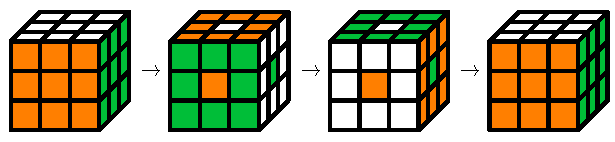
\includegraphics[width=10cm]{rubikrot-doc-figC.pdf}
% \else
% \fi
% \end{minipage}
%
%
%   \subsubsection{Random rotations}
%
%  The \cmd{\RubikRotation} command  can also be used to  scramble the 
% cube using a random sequence of rotations. If  the first argument 
% is the lower-case word `random' \textsc{and} the second argument 
% is an integer $n$, ($1\leq n \leq 200$), then a random sequence 
% of $n$ rotations will be performed; otherwise  a default value 
% of 50 is used (for example, if the second argument is not an integer). 
% If $n > 200$ then  the currently set maximum value $n=200$ will be used.
%
%  As a safety feature the  maximum $n$ can be changed only by editing  the 
%  set value of  the Perl variable \verb!$maxn! in the Perl script 
%  \texttt{rubikrotation.pl},  where we  currently have
%  (see  the `random' subroutine in the document \texttt{rubikrotationPL.pdf})
%\begin{quote}
%\begin{verbatim}
% my $maxn=200;
%\end{verbatim}
%\end{quote}
%
% For example, the following commands scramble a solved cube using a 
% sequence of 120 random rotations, and display the state in the form of 
%  a  semi-flat (SF) cube. 
%

% \begin{minipage}{3.4cm}
% \centering
% \ifpdf
%   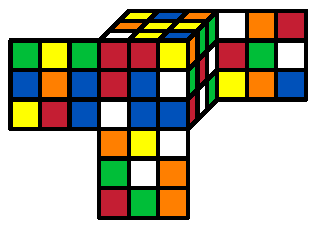
\includegraphics[height=4cm]{rubikrot-doc-figB.pdf}
% \else
% \fi
% \end{minipage}
% \begin{minipage}{6cm}
% \vspace{1.6cm}
%\begin{verbatim}
% \RubikCubeSolved%
% \RubikRotation{random,120}%
% \ShowCube{5.5cm}{0.5}{\DrawRubikCubeSF}
%\end{verbatim}
% \end{minipage}
%
% Note that in this particular example (above), only 
% the \cmd{\Draw..} command is inside the TikZ picture environment (i.e.,~inside 
% the \cmd{\ShowCube} command). Note also that when Rubik
% commands are outside a TikZ picture environment, they should have a 
% trailing \% to stop additional white space being included.
%
% \medskip
%
% The randomisation procedure is as follows: all the possible rotations  are first allocated 
% a different cardinal number (positive integer) and collected into an  array. 
%  Then  a  sequence of $n$ randomised numbers is generated and  mapped to 
% the array  to generate the associated sequence of random rotations. 
% The sequence used is detailed in the \texttt{.log} file.
%
%
%  \subsection[SaveRubikState]{\cmd{\SaveRubikState} command}
% \label{saverubikstate}
%
%  \DescribeMacro{\SaveRubikState}
%  The command  \cmd{\SaveRubikState}\marg{filename} saves the state (configuration) 
%  of the Rubik cube to  the file  \marg{filename} in the standard \cmd{\RubikFace...}
%  format so that it can be read by \LaTeX. Consequently such a file can then be input 
%  so it can be drawn or processed in the usual way. The output file is `closed' immediately
%  following the `write' in order to allow it to be available for input later by the same 
%  file if required.
%
% For example, the following commands would save the so-called `sixspot' configuration
%  (generated by the rotations \textbf{U, Dp, R, Lp, F, Bp, U, Dp})
% to the file \verb!sixspot.tex!.
%\begin{quote}
%\begin{verbatim}
% \RubikCubeSolved%
% \RubikRotation{U,Dp,R,Lp,F,Bp,U,Dp}%
% \SaveRubikState{sixspot.tex}%
%\end{verbatim}
%\end{quote}
% The form of the  file \verb!sixspot.tex! will then be as follows---the 
% filename (commented out) is automatically written to the  top of the 
% file for convenience.
%\begin{quote}
%\begin{verbatim}
% % filename: sixspot.tex
% \RubikFaceUp{O}{O}{O}{O}{W}{O}{O}{O}{O}%
% \RubikFaceDown{R}{R}{R}{R}{Y}{R}{R}{R}{R}%
% \RubikFaceLeft{Y}{Y}{Y}{Y}{B}{Y}{Y}{Y}{Y}%
% \RubikFaceRight{W}{W}{W}{W}{G}{W}{W}{W}{W}%
% \RubikFaceFront{G}{G}{G}{G}{O}{G}{G}{G}{G}%
% \RubikFaceBack{B}{B}{B}{B}{R}{B}{B}{B}{B}%
%\end{verbatim}
%\end{quote}
% We can therefore access and draw this configuration in a Semi-Flat  format 
% later, when required,  simply by inputting  the file as follows:
%\begin{quote}
%\begin{verbatim}
%\input{sixspot.tex} 
%\ShowCube{7cm}{0.7}{\DrawRubikCubeSF}
%\end{verbatim}
%\end{quote}
%
%
%  \subsection[CheckRubikState]{\cmd{\CheckRubikState} command}
%
%  \DescribeMacro{\CheckRubikState}
%  Since it is easy to inadvertently define an invalid Rubik cube 
% (e.g.,~enter an invalid number of, say, yellow facelets), this command 
%  simply checks the current colour state of all the cubies
% of a 3x3x3 Rubik cube, and  shows the number of facelets  of each colour.  
% An ERROR: code is issued if the number of facelets having a given colour exceeds~6.
% The results are written to the the \texttt{.log} file, and displayed under 
% the graphic if the \cmd{\ShowRubikErrors} command is used.
%
% One can check the current Rubik state (for errors) by issuing  the command
%\begin{quote}
%\begin{verbatim}
% \CheckRubikState%
%\end{verbatim}
%\end{quote}
% Note (1)~that  such a check is implemented automatically with each \cmd{\RubikRotation} 
% command, and (2)~this is actually only a very superficial check---simply counting the number 
% of cubies of each colour.
%
%
%
%
%   \subsection[ShowRubikErrors]{\cmd{\ShowRubikErrors} command}
%
%   \DescribeMacro{\ShowRubikErrors}
% Any errors which arise  can be made visible using  the 
% command  \cmd{\ShowRubikErrors}. 
% This command  places a copy of the `error' file (\texttt{rubikstateERRORS.dat})  
% underneath the graphic image so you can see any errors if there are any---all this 
% detail can also be found in the \texttt{.log} file. 
%
%  Consequently, this  command must be placed \textit{after} a TikZ picture 
%  environment---it cannot be used  inside a TikZ environment. In fact this command 
%  is probably best placed at the  end of the document (if there are several such 
%  environments), where it will reveal  all rotation errors  generated while 
%  processing the whole document.
% Once the document is free of errors this command can be removed or just commented out. 
% Run the test file \texttt{example-rot.tex} to see an example of the use of this command. 
%
%
%    \section{Files generated}
%
% 
% Whenever the \cmd{\RubikRotation} or \cmd{\CheckRubikState} commands are used, 
% three small temporary  plain-text files for holding data are generated  as 
% follows (they are refreshed with each \LaTeX\ run, and are not actively deleted).
% \begin{itemize}
% \item  \LaTeX\ writes Rubik state data to the file \texttt{rubikstate.dat}.
%
% \item  The Perl script \texttt{rubikrotation.pl} reads the file
% \texttt{rubikstate.dat} and then   writes 
%  the new rubik state to the file \texttt{rubikstateNEW.dat}.
%
% \item   The Perl script \texttt{rubikrotation.pl} also writes error data 
% to the file \texttt{rubikstateERRORS.dat}.  A copy of this file is  displayed 
% under the graphic image  when the command 
% \cmd{\ShowRubikErrors} is used after  the TikZ picture environment.
%
% \end{itemize}
%
% 
%     \section{General overview}
%   \label{generaloverview}
%
%  When \LaTeX\  processes  \texttt{rubikrotation.sty}  the following steps
%  are implemented.
% \begin{itemize}
% 
% \item[1.]  A check is made to see if  \texttt{fancyvrb.sty} is loaded: if not 
% then this package  is loaded  (this package supplies the command \cmd{\VerbatimInput} which 
% is required for inputting the  file  \texttt{rubikstateERRORS.dat} in verbatim form).
% 
% \item[2.]  A check is made to see if a configuration-file (\texttt{rubikrotation.cfg})
%  exists:  if so then  this file is input.
%
% \item[3.] The text file \texttt{rubikstateNEW.dat} is overwritten (if it exists), 
%  otherwise the file is created (this prevents an `old' version of the file being 
%  used by \LaTeX).
%
% \item[4.]  The plain-text file \texttt{rubikstateERRORS.dat} is created. 
% This file collects error  messages generated by the Perl script.
%
% \end{itemize}
%
%
% When a \cmd{\RubikRotation} command is processed it first  writes the current 
% colour configuration of each face (the `rubik state') to the temporary file 
% \texttt{rubikstate.dat} (this will be read by the Perl script \texttt{rubikrotation.pl}). 
% The \cmd{\RubikRotation} command also appends the keyword `\texttt{checkrubik}' 
%  as well as  a copy of the  string of Rubik rotations. 
% It~then calls the Perl script  \texttt{rubikrotation.pl}. 
%
% For example, if we use the command \cmd{\RubikCubeSolved}
% followed by the command \verb!\RubikRotation[2]{U,D,L,R}!, then the associated 
%  \texttt{rubikstate.dat} file  will be written as follows:
%\begin{quote}
% \begin{verbatim}
% % filename: rubikstate.dat
% up,W,W,W,W,W,W,W,W,W
% down,Y,Y,Y,Y,Y,Y,Y,Y,Y
% left,B,B,B,B,B,B,B,B,B
% right,G,G,G,G,G,G,G,G,G
% front,O,O,O,O,O,O,O,O,O
% back,R,R,R,R,R,R,R,R,R
% checkstate
% rotation,U,D,L,R
% rotation,U,D,L,R
%\end{verbatim}
%\end{quote}
% Note that the \cmd{\RubikRotation} option \texttt{[2]} results in the string ``\texttt{rotation,U,D,L,R}'' 
% being written twice to the \texttt{rubikstate.dat} file, as shown above.
%
% Alternatively, if we used the command 
% \verb!\RubikRotation{random, 45}! then the last line  written to the file 
% would be the string  ``\texttt{rotation,random,45}'', as follows:
%\begin{quote}
% \begin{verbatim}
% % filename: rubikstate.dat
% up,W,W,W,W,W,W,W,W,W
% down,Y,Y,Y,Y,Y,Y,Y,Y,Y
% left,B,B,B,B,B,B,B,B,B
% right,G,G,G,G,G,G,G,G,G
% front,O,O,O,O,O,O,O,O,O
% back,R,R,R,R,R,R,R,R,R
% checkstate
% rotation,random,45
%\end{verbatim}
%\end{quote}
% A  \cmd{\CheckRubikState} command   triggers the same sequence of events except
% that no ``\texttt{rotation,....}'' line is written.
%
% The action of the Perl script  \texttt{rubikrotation.pl} is controlled by 
% the keywords (first argument of
% each line)  associated with each line of the file \texttt{rubikstate.dat}. 
% When control passes to  Perl,  the script \texttt{rubikrotation.pl} starts 
% by loading the current rubikstate (prompted by the keywords `\texttt{up}', `\texttt{down}', 
% `\texttt{left}', `\texttt{right}', `\texttt{front}', `\texttt{back}'), and performing
% a syntax check---significant syntax errors at this stage 
%  will cause the program to  issue appropriate error messages and then terminate cleanly.
% Next, the Perl script  performs  some basic cube checks 
% (prompted by the key word `\texttt{checkstate}'), and then the program processes  
% the sequence of Rubik rotations (prompted by the keyword 
% `\texttt{rotation}').  If, instead, the second argument  of the `\texttt{rotation,...}' string 
% is the keyword `\texttt{random}', and  provided this is followed by a valid integer, say $n$, 
% then the Perl script performs  a sequence of $n$ random rotations.
% Finally, the Perl script writes the final rubikstate to the text file 
% \texttt{rubikstateNEW.dat}. All error messages are written to the 
% text file \texttt{rubikstateERRORS.dat} and  also to the \LaTeX\  log-file. 
%
% Control then reverts to  \LaTeX\  which then inputs the file
% \texttt{rubikstateNEW.dat}. If there are more \cmd{\RubikRotation} commands
% (in the \texttt{.tex} file) then this cycle  repeats accordingly.  
% Eventually a \cmd{\Draw...} command is  reached (in the \texttt{.tex} file) and 
% the final rubikstate is drawn in a TikZ picture  environment.
%
% If the TikZ picture environment is followed by a \cmd{\ShowRubikErrors} command,
% then a `verbatim' copy of the \texttt{rubikstateERRORS.dat} file is displayed
% immediately under the graphic. Once the graphic is error-free, then the
% \cmd{\ShowRubikErrors} command can be removed or commented out. 
%
% Note that if a \textsc{bash}  file is used to coordinate the process then it is often
% convenient to use the linux \texttt{grep} utility to alert the user to any run-time errors,
% by using \texttt{grep} to scan the   \texttt{rubikstateERRORS.dat} file at the end of 
% the run; for example, as follows:
%\begin{quote}
%\begin{verbatim}
% pdflatex  --shell-escape  myfile.tex
% echo "...checking error file" 
% grep ERROR  ./rubikstateERRORS.dat
%\end{verbatim} 
%\end{quote}
%
%
%   \section{References}
%     \label{sec:references}
%
%\begin{itemize}
%
% \item Abrahams PW, Berry K and Hargreaves KA (1990).  \textit{\TeX\ for the impatient} 
% (Addison-Wesley Publishing Company), page~292.   
% {\newline}Available from: \url{http://www.ctan.org/pkg/impatient}
% {\newline}[\,re:~\cmd{\rubikpercentchar}  and  \cmd{\@comment} in Section~\ref{sec:abrahams}\,]
%
%
% \item Eijkhout V (1992). \textit{\TeX\ by topic: a {\TeX}nician's reference}.
% (Addison-Wesley Publishing Company), pages~232 \&~238. 
% {\newline}Available from:  \url{https://bitbucket.org/VictorEijkhout/tex-by-topic/}
% [\,re:~\cmd{\string} in Section~\ref{sec:eijkhout}\,]
% [\,re:~\cmd{\write} in Section~\ref{sec:seq-as-macros}\,]
%
%
% \item Feuers\"{a}nger C (2015). Notes on programming in \TeX. 
% {\newline}(revision: 1.12.1-32-gc90572c; 2015/07/29) 
% \newline\url{http://pgfplots.sourceforge.net/TeX-programming-notes.pdf}
% {\newline}[\,re:~loop macros in Section~\ref{sec:feuersanger}\,]
%
%  \item Kociemba  website (Kociemba H). \url{http://www.kociemba.org/cube.htm}
%
% \item Nickalls RWD and Syropoulos A (2015).  The \textsc{rubikcube} package, v3.0.
% \newline\url{http://www.ctan.org/pkg/rubik}, 
%
%
% \item Randelshofer website (Randelshofer W).  \url{http://www.randelshofer.ch/rubik/}
%  \ [\,re:~sequences  and  supersetENG notation\,]
%
%
% \item Reid website (Reid M). \  Patterns.  \url{http://www.cflmath.com/Rubik/patterns.html}
% \ [\,re:~sequences as macros; in Section~\ref{sec:seq-as-macros}\,]
%
%
% \item Tellechea C and Segletes SB (2016).  The  \textsf{listofitems} package, v1.2
% \newline\url{http://www.ctan.org/pkg/listofitems}
%\end{itemize}
% 
%
%
%     \section{Change history}
%
% \begin{itemize}
%
% \item Version 4.0 (March  2017)
%
% --- The \cmd{\RubikRotation} command has been enhanced to allow its argument to include
%  so-called repeat-blocks (rotation-sequences which can be repeated multiple times), and 
% info-blocks for holding sequence metadata (see Section~\ref{sec:rubikrotationcmd}).
% Syntax checking of the \cmd{\RubikRotation} argument is much improved 
% (see \texttt{rubikrotationPL.pdf} for details of the Perl script).
%
% --- Four new macros  which  hold derived data (see Section~\ref{sec:rubikrotationcmd}).
% \begin{quote}
%  \cmd{\SequenceName}
%  \newline\cmd{\SequenceInfo}
%  \newline\cmd{\SequenceShort}
%  \newline\cmd{\SequenceLong}
% \end{quote}
%
% --- Better syntax checking of the \cmd{\RubikRotation} argument by the Perl program \texttt{rubikrotation.pl}.
%
%
%
% \item Version 3.0 (25 September 2015)
%
% --- The \cmd{\RubikRotation} command now  actions multiple instances of its  argument 
% as determined by an optional `repeat' \oarg{integer}. For example  the command 
% \cmd{\RubikRotation[3]\{R,x\}}  is equivalent to the  command \cmd{\RubikRotation\{R,x,R,x,R,x\}}
% (see Sections~\ref{sec:rubikrotationcmd} and \ref{sec:rubikrotationcode}).
%
% --- If a comma separated  element used as an argument for the \cmd{\RubikRotation} 
% command is prefixed with either a * or [ or ]  character then it is not actioned 
% as a rotation (see Section~\ref{sec:prefixedargument}). 
%
% --- The Perl script \texttt{rubikrotation.pl} now has command-line switches, 
% including \texttt{-h} to show some `help'  and `usage' information 
% (see Section~\ref{sec:placingfiles}).
%
% --- A `man' file (manual file) for the Perl script \texttt{rubikrotation.pl} is now 
%  included in the package.
%
% --- The Perl script \texttt{rubikrotation.pl} now  uses as input and output filenames
%  those specified  in the command-line of the CALLing program. This now allows the 
%  script \texttt{rubikrotation.pl} to be used as a stand-alone tool (see the
%  \texttt{rubikrotation}  `man' file for details).
%
% --- The documentation for the Perl script \texttt{rubikrotation.pl} is in the
% accompanying file \texttt{rubikrotationPL.pdf}.
% 
% --- Fixed  typos, index and minor errors in the documentation. 
%
%
% \item Version 2.0 (5 February, 2014)
%
% --- First release.
%
% \end{itemize}
%
% ^^A ==================================================
% \StopEventually{\PrintIndex}
%
%
%
%        \section[The code]{The code (\texttt{rubikrotation.sty})} 
% 
% {\noindent}In the following, the term `Perl script'  denotes the script
%  \texttt{rubikrotation.pl}. Useful information regarding the 
% \TeX\  \cmd{\write} command  is given in Eijkhout (1992), \S\,30.2.3 (page~238). 
%  For the means of including a `\%' character in the token list of \cmd{\write} see 
%  Abrahams \textit{et.~al} (1990).
% 
%   \subsection{Package heading}
%   \label{sec:CodePackageHeading}
%
%    \begin{macrocode}
%<*rubikrotation>
\def\RRfileversion{4.0}%
\def\RRfiledate{2017/03/03}%
\NeedsTeXFormat{LaTeX2e}
\ProvidesPackage{rubikrotation}[\RRfiledate\space (v\RRfileversion)]
%    \end{macrocode}
%
%
% {\noindent}The package requires \texttt{rubikcube.sty}. However \texttt{rubikcube.sty}
% is not automatically loaded (for the moment at least) since this makes it difficult 
% to errorcheck new versions.
%    \begin{macrocode}
\@ifpackageloaded{rubikcube}{}{%
   \typeout{---rubikrotation requires the rubikcube package.}%
   }%
%    \end{macrocode}
%
%
%
%  {\noindent}The \rubikrotation\  package requires access to the  \textsf{fancyvrb} package
%  for the \cmd{\VerbatimInput\{\}} command  which we use for inputting and displaying
%  the error file (see Section~\ref{sec:showrubikerrors}).
%    \begin{macrocode}
\@ifpackageloaded{fancyvrb}{}{%
   \typeout{---rubikrotation requires the fancyvrb package%
       for VerbatimInput{} command.}%
   \RequirePackage{fancyvrb}}
%    \end{macrocode}
%
%
%   {\noindent}For the \cmd{\write18} syntax to work with
%   Lua\TeX\ (so we can access system commands) we require 
%   the recent \textsf{shellesc} package, which we load using the 
%   \textsf{ifluatex} conditional (see Section~\ref{sec:shellescape}).
%    \begin{macrocode}
\@ifpackageloaded{ifluatex}{}{%
   \typeout{---rubikrotation requires the ifluatex package.}%
   \RequirePackage{ifluatex}}
\ifluatex%
   \@ifpackageloaded{shellesc}{}{%
   \typeout{---rubikrotation requires the shellesc package
       to run using Lua\LaTeX.}%
   \RequirePackage{shellesc}}
\fi%
%    \end{macrocode}
%
%
%  \medskip
% 
%   \subsection{Some useful commands}
%   \label{sec:usefulcommands}
%
%    \begin{macro}{\rubikrotation}
% First we create a suitable logo
%    \begin{macrocode}
\newcommand{\rubikrotation}{\textsc{rubikrotation}}
\newcommand{\Rubikrotation}{\textsc{Rubikrotation}}
%    \end{macrocode}
%    \end{macro}
%
%
%
%    \begin{macro}{\@print}
% We need  a simple print command to facilitate writing output to a file.
%    \begin{macrocode}
\newcommand{\@print}[1]{\immediate\write\outfile{#1}}
%    \end{macrocode}
%    \end{macro}
%
%
%
%    \begin{macro}{\@comment}
%    \begin{macro}{\@commentone}
%  We also require  access to the `\%' character so we can (a)~write comments to
%  files, including the log file, and (b)~place a  trailing `\%' in a line of code
%  written to a file.
%
%  To achieve this we define the `\%' character  as \cmd{\rubikpercentchar} 
%  (modified from:  Abrahams PW, Berry K and Hargreaves KA (1990), p~292)
% [see refs Section~\ref{sec:references}]\label{sec:abrahams}, 
% and also two `comment' commands which implement it. This `workaround'
% is necessary because \TeX\ does not allow the use of  the \cmd{\%} command 
% for placing a  `\%' character in the token list of \cmd{\write}. 
% See Abrahams \textit{et.~al} (1990) for details.
%    \begin{macrocode}
{\catcode`\%=12   \global\def\rubikpercentchar{%}}%
\newcommand{\@comment}{\rubikpercentchar\rubikpercentchar\space}%
\newcommand{\@commentone}{\rubikpercentchar}%
%    \end{macrocode}
%    \end{macro}
%    \end{macro}
%
%
%
%    \begin{macro}{\rubikperlname}
%  This holds the name of the Perl script.  A configuration-file
% (\verb!rubikrotation.cfg!) can be used to change the default name of the 
% Perl script using a renewcommand (see Section~\ref{sec:configfile}). 
%    \begin{macrocode}
\newcommand{\rubikperlname}{rubikrotation}
%    \end{macrocode}
%    \end{macro}
% Note that here we are assuming that the script is an executable file.
%
%    \begin{macro}{\rubikperlcmd}
%  This holds the command-line  code for calling the Perl script 
%  Note that the command-line requires a mandatory  input filename preceded
%  by the \texttt{-i}~switch. An optional output filename (preceded by the
%  \texttt{-o}~switch) may be used, otherwise the default output filename of 
%  \texttt{rubik-OUT.dat} will be used.
%
% Note that it is very important that we do actually specify an
% output filename (for receiving data from the Perl script). This is because
% (a)~The Perl script \texttt{rubikrotation.pl} is currently configured to read its 
% output filename  as an argument from the command-line (so it can be flexibly 
% used as a stand-alone script for processing a given Rubik state through a 
% sequence of rotations), and (b)~\texttt{rubikrotation.sty} is currently 
% configured to read  its input (i.e.,~data  generated  by  the Perl script)
%  from the file \texttt{rubikstateNEW.dat}.
%    \begin{macrocode}
\newcommand{\rubikperlcmd}{\rubikperlname\space%
                   -i rubikstate.dat   -o rubikstateNEW.dat}
%    \end{macrocode}
%  Remember to use the \cmd{\space} macro following the \cmd{\rubikperlname} macro 
%  in order to  generate the mandatory space before the first 
% command-line argument.
%
%  A plain-text  configuration-file \verb!rubikrotation.cfg! can be used to 
%  change the default command-line code  using a renewcommand 
%  (see Section~\ref{sec:configfile}). 
%    \end{macro}
%
%
%     \subsection{Configuration file}
%
% If a configuration file exists (\texttt{rubikrotation.cfg}) then input it here,
% i.e.,~\textit{after} defining the \cmd{\rubikperlname} and \cmd{\rubikperlcmd} 
% macros and \textit{before} creating the \texttt{rubikstateERRORS.dat} file.
%    \begin{macrocode}
\typeout{---checking for config file (rubikrotation.cfg)...}
\IfFileExists{rubikrotation.cfg}{%
   %% rubikrotation.ins 
%%
%% version 4.0
%%
%% --- automatic overwriting of .sty is disabled-------
%%  =========================================================
%%
%% --------------- start of docstrip commands ------------------
%%
\def\batchfile{rubikrotation.ins}
\input docstrip.tex

\preamble

----------------------------------------------------------------- 
  Authors: RWD Nickalls (dick@nickalls.org) 
          and Apostolos Syropoulos (asyropoulos@yahoo.com)

  Copyright 03 March 2017     RWD Nickalls and A Syropoulos

  VERSION 4.0

  This work may be distributed and/or modified under the
  conditions of the LaTeX Project Public License, either
  version 1.3c of this license or (at your option) any 
  later version: <http://www.latex-project.org/lppl.txt>

  This work consists of the files listed in the README file.
----------------------------------------------------------------- 

  This is a LaTeX/TikZ package for drawing Rubik cubes
  Please report errors or suggestions for improvement to

         RWD Nickalls  (dick@nickalls.org)
         Apostolos Syropoulos (asyropoulos@yahoo.com)

 This package requires the basic TikZ package to be loaded already
------------------------------------------------------------------
\endpreamble

\keepsilent  %%disables most of the screen output
%% \askforoverwritefalse  %%enables automatic overwriting of .sty 
\generate{\file{rubikrotation.sty}{\from{rubikrotation.dtx}{rubikrotation}}}

%%now write a screen message for the user
\obeyspaces
\Msg{*******************************************************}
\Msg{*                                                     *}
\Msg{* To finish the installation you have to move the     *}
\Msg{* following file into a directory searched by TeX:    *}
\Msg{*                                                     *}
\Msg{*       rubikrotation.sty                             *}
\Msg{*                                                     *}
\Msg{* To produce the documentation run the file           *}
\Msg{* rubikrotation.dtx through LaTeX.                    *}
\Msg{* For an index, process any filename.idx  file by     *}
\Msg{*      makeindex -s gind.ist filename                 *}
\Msg{* For list of changes, process any filename.glo file  *}
\Msg{* makeindex -s gglo.ist -o filename.gls filename.glo  *}
\Msg{*                                                     *}
\Msg{* Happy TeXing!                                       *}
\Msg{*******************************************************}

\endbatchfile
%%------------EOF---------------
%
   }{\typeout{---no config file available}%
}%
%    \end{macrocode}
%
%
%   \subsection{Clean file rubikstateNEW.dat}
%
% {\noindent}We need to clean out any existing (old) rubikstateNEW.dat file,
% since if the TeX shell command-line switch is accidentally not used then the Perl script 
% \texttt{rubikrotation.pl} will not be CALLed,  and hence this file will not be renewed 
% (i.e.,~an `old' image may be used).
%    \begin{macrocode}
\typeout{---cleaning file rubikstateNEW.dat}%
\newwrite\outfile%
\immediate\openout\outfile=rubikstateNEW.dat%
\@print{\@comment rubikstateNEW.dat}%
\immediate\closeout\outfile%
%    \end{macrocode}
%
%
%   \subsection{rubikstateERRORS.dat}
%
%  {\noindent}We first  open the file \texttt{rubikstateERRORS.dat} which is used
% by the Perl script \texttt{rubikrotation.pl} for writing its error-messages to.  
% This file is displayed by the command 
% \cmd{\ShowRubikErrors}.
%
%  \textsc{important note}: this file is created fresh each time LaTeX is run,
%  and hence the Perl  script  only appends data to it during the \LaTeX\ run,
%  so this file just grows until either it is  destroyed or recreated---this is
%  a useful feature since the file  accumulates all error messages as the 
% \texttt{.tex} file is processed.
%  We can't make the Perl  script  create the file  since the Perl script is only 
% CALLed if we  use a  \cmd{\RubikRotation} or \cmd{\CheckRubikState} 
% command (which we may not\,!)---so it  has to be created here.
%    \begin{macrocode}
\typeout{---creating file rubikstateERRORS.dat}%
\newwrite\outfile%
\immediate\openout\outfile=rubikstateERRORS.dat%
\@print{\@comment rubikstateERRORS.dat}%
\@print{\@comment --------------------}%
\immediate\closeout\outfile%
%    \end{macrocode}
%
%
%    \subsection{Setting up file-access for new files}
% 
%  Having set up all the primary files, we now need to set up  a newwrite for 
% all subsequent file openings (e.g.,~for \texttt{rubikstate.dat} and  saving 
% to arbitrary filenames by the \cmd{\SaveRubikState} command). Otherwise, we 
% can easily exceed the LaTeX limit of 15. From here-on  \TeX\ will use 
% \texttt{openout7} when opening and writing to files. We will implement new 
% openings using the command \verb!\@openstatefile! (see below). 
%    \begin{macrocode}
\typeout{---setting up newwrite for rubikrotation.sty to use...}%
\newwrite\outfile%
%    \end{macrocode}
%
%
%    \begin{macro}{\@openstatefile}
%    \begin{macro}{\@closestatefile}
% We also need   commands for easy file opening and  closing
% for new instances of the file \texttt{rubikstate.dat} etc.
% Note that for this we are therefore using the same outfile number as set up
% by the \verb!\newwrite...!  above. 
%    \begin{macrocode}
\newcommand{\@openstatefile}{\immediate\openout\outfile=rubikstate.dat}
\newcommand{\@closestatefile}{\immediate\closeout\outfile}
%    \end{macrocode}
%    \end{macro}
%    \end{macro}
%
%
%    \subsection{Saving the Rubik state}
%
%    \begin{macro}{\@printrubikstate}
% This internal command  writes the Rubik configuration to
% the file \texttt{rubikstate.dat}, and is used by the \cmd{\RubikRotation} command
% (see Sections~\ref{saverubikstate} and \ref{generaloverview}).
%  The file \texttt{rubikstate.dat} is read by the Perl script, and represents 
% the state on which  the new \cmd{\RubikRotation} command acts.
% Note that we append the key-word \texttt{checkstate} to the end of the file
% in order to trigger the Perl script to implement its \texttt{checkstate} subroutine.
%
% The actual state is simply an ordered sequence of the  faces and the colours 
% associated with each facelet of a face. The colour associated with a particular facelet
% is held by the variable for that facelet. For example, the top-left facelet associated with
% the \textsc{front} face is held in the variable \cmd{\Flt} (see Section~\ref{saverubikstate}).
% Further relevant documentation is in the \textsc{rubikcube} package. 
%    \begin{macrocode}
\newcommand{\@printrubikstate}{%
   \@print{up,\Ult,\Umt,\Urt,\Ulm,\Umm,\Urm,\Ulb,\Umb,\Urb}%
   \@print{down,\Dlt,\Dmt,\Drt,\Dlm,\Dmm,\Drm,\Dlb,\Dmb,\Drb}%
   \@print{left,\Llt,\Lmt,\Lrt,\Llm,\Lmm,\Lrm,\Llb,\Lmb,\Lrb}%
   \@print{right,\Rlt,\Rmt,\Rrt,\Rlm,\Rmm,\Rrm,\Rlb,\Rmb,\Rrb}%
   \@print{front,\Flt,\Fmt,\Frt,\Flm,\Fmm,\Frm,\Flb,\Fmb,\Frb}%
   \@print{back,\Blt,\Bmt,\Brt,\Blm,\Bmm,\Brm,\Blb,\Bmb,\Brb}%
   \@print{checkstate}%
}
%    \end{macrocode}
%    \end{macro}
%
%
% \subsection{SaveRubikState command}
% \label{sec:eijkhout}
%
% \begin{macro}{\SaveRubikState} 
% The command \cmd{\SaveRubikState}\marg{filename} saves the Rubik state
% to a named file in the format of a Rubik command (so it can then be processed
% by \LaTeX).  Note that in order to actually write  a LaTeX
% command to a file without a trailing space one must prefix the command with  the 
%  \cmd{\string} command (see Eijkhout (1992), p~238) 
% [see refs Section~\ref{sec:references}]\label{sec:eijkhout}. 
%
% Note that this macro uses the  internal commands \cmd{\@comment} (`\%\%'), 
% \cmd{\@commentone} (`\%')  and \cmd{\@print}.  \#1 is the output filename.
% We use several \cmd{\typeout} commands to write to the log file.
% An example of the line of code  we are trying to output to the 
%\texttt{rubikstateNEW.dat} file  is as follows:
% {\newline}\verb!\RubikFaceUp{W}{W}{G}{W}{W}{G}{B}{B}{Y}%! 
%    \begin{macrocode}
\newcommand{\SaveRubikState}[1]{%
\typeout{---NEW save command------------------}%
\typeout{---command = SaveRubikState{#1}}%
\typeout{---saving Rubik state data to file #1}%
\immediate\openout\outfile=#1%
\@print{\@comment filename: #1\@commentone}%
\@print{\string\RubikFaceUp%
   {\Ult}{\Umt}{\Urt}{\Ulm}{\Umm}{\Urm}{\Ulb}{\Umb}{\Urb}\@commentone}%
\@print{\string\RubikFaceDown%
   {\Dlt}{\Dmt}{\Drt}{\Dlm}{\Dmm}{\Drm}{\Dlb}{\Dmb}{\Drb}\@commentone}%
\@print{\string\RubikFaceLeft%
   {\Llt}{\Lmt}{\Lrt}{\Llm}{\Lmm}{\Lrm}{\Llb}{\Lmb}{\Lrb}\@commentone}%
\@print{\string\RubikFaceRight%
   {\Rlt}{\Rmt}{\Rrt}{\Rlm}{\Rmm}{\Rrm}{\Rlb}{\Rmb}{\Rrb}\@commentone}%
\@print{\string\RubikFaceFront%
   {\Flt}{\Fmt}{\Frt}{\Flm}{\Fmm}{\Frm}{\Flb}{\Fmb}{\Frb}\@commentone}%
\@print{\string\RubikFaceBack%
   {\Blt}{\Bmt}{\Brt}{\Blm}{\Bmm}{\Brm}{\Blb}{\Bmb}{\Brb}\@commentone}%
\immediate\closeout\outfile%
\typeout{-----------------------------------------}%
}%
%    \end{macrocode}
%  \end{macro}
%
%
%    \subsection{RubikRotation command}
%   \label{sec:rubikrotationcode}
%
%    \begin{macro}{\RubikRotation}
% The \cmd{\RubikRotation}\oarg{integer}\marg{comma separated sequence} 
% command (a)~writes the current Rubik state to the file \texttt{rubikstate.dat},
% (b)~writes the rotation sequence (either once or multiple times depending 
% on the value of the optional integer argument), and then (c)~CALLs the 
% Perl script \texttt{rubikrotation.pl}.  It~also writes comments to the 
% data file and also to the log file.
%
% The way we allow the user to (optionally) process the main argument multiple
%  times  is simply by writing the associated output command multiple
% times to the output data-file. Consequently, we require the \cmd{\RubikRotation} 
% command to allow a square-bracket optional
% argument (a non-negative integer) to specify the number of such repeats.
% In order to implement this optional argument facility we use two macros 
% (countingloop and loopcounter) detailed by Feuers\"{a}nger (2015) 
% [\,see refs Section~\ref{sec:references}\,]\label{sec:feuersanger}, 
% as follows:
%    \begin{macrocode}
%% Two macros detailed by Feuersaenger (2015)
\long\def\@countingloop#1 in #2:#3#4{%
   #1=#2 %
   \@loopcounter{#1}{#3}{#4}%
}
%%--------------------------
\long\def\@loopcounter#1#2#3{%
   #3%
   \ifnum#1=#2 %
        \let\next=\relax%
   \else
        \advance#1 by1 %
        \def\next{\@loopcounter{#1}{#2}{#3}}%
   \fi
   \next
}
%    \end{macrocode}
% Having defined the above two macros we can now implement an optional
% argument (a repeat number) indicating the number of times we want 
% the command to write the main argument to the output data file.
%    \begin{macrocode}
\newcommand{\RubikRotation}[2][1]{%
   \typeout{---TeX process (rubikrotation.sty)-------}% 
   \typeout{---NEW rotation command------------------}%
   \typeout{---command = RubikRotation[#1]{#2}}%
   \typeout{---writing current Rubik state to file rubikstate.dat}%
   \@openstatefile% open data file
   \@print{\@comment filename: rubikstate.dat}%
   \@print{\@comment written by rubikrotation.sty%
                         =v\RRfileversion\space (\RRfiledate)}%
   \@printrubikstate% 
%% countingloop code from Feuersaenger (2015)
   \newcount\ourRRcounter%
   \@countingloop{\ourRRcounter} in 1:{#1}{%
         \immediate\write\outfile{rotation,#2}}%
   \@closestatefile% close data file
   \typeout{---CALLing Perl script (rubikrotation.pl)}%
   \immediate\write18{\rubikperlcmd}%
   \typeout{---inputting NEW datafile (data written by Perl script)}%
   \input{rubikstateNEW.dat}%
   \typeout{-----------------------------------------}%
 }
%    \end{macrocode}
%    \end{macro}
% Note that the new \cmd{\ShellEscape} command implemented by the recent
% \textsf{shellesc} package is equivalent to \cmd{\immediate}\cmd{\write18} (see above),
%  and so we  probably ought to use \cmd{\ShellEscape} instead in future (and hence load
% \textsf{shellesc} automatically). At present, however, we leave the user to make 
% sure that the \textsf{shellesc} package is actually  available on their system.
% 
%
%
%   \subsection{ShowRubikErrors command}
%  \label{sec:showrubikerrors}
%
%    \begin{macro}{\ShowRubikErrors}
% This command inputs the file \texttt{rubikstateERRORS.dat}.
% Also made a more convenient synonym = \cmd{\ShowErrors}.
%    \begin{macrocode}
\newcommand{\ShowRubikErrors}{%
   \typeout{---ShowRubikErrors: inputting file rubikstateERRORS.dat}%
   \VerbatimInput{rubikstateERRORS.dat}%
 }
\newcommand{\ShowErrors}{\ShowRubikErrors}
%    \end{macrocode}
%    \end{macro}
%
%
%   \subsection{CheckRubikState command}
%
%    \begin{macro}{\CheckRubikState}
% This command triggers the Perl script to implement 
%  some simple error checking of the Rubik configuration (state).
% This command (a)~writes the current Rubik state to the file 
% \texttt{rubikstate.dat}, and then (b)~CALLs the Perl script.
% It also writes comments to the data file and also to the  log file..
%    \begin{macrocode}
\newcommand{\CheckRubikState}{%
   \typeout{---NEW check command------------------}%
   \typeout{---command = CheckRubikState}%
   \typeout{---writing current Rubik state to file rubikstate.dat}%
   \@openstatefile% opens data file
   \@print{\@comment filename: rubikstate.dat}%
   \@printrubikstate% 
   \@closestatefile% close data file
   \typeout{---running Perl script (rubikrotation.pl)}%
   \immediate\write18{\rubikperlcmd}%
   \typeout{---inputting NEW datafile (data written by Perl script)}%
   \input{rubikstateNEW.dat}%
   \typeout{-----------------------------------------}%
 }
%    \end{macrocode}
%    \end{macro}
%
%
% --------------------------
%    End of this package
% --------------------------
%    \begin{macrocode}
%</rubikrotation>
%    \end{macrocode}
%
%
%
%
% \Finale
%
\endinput





